\subsection[Diseño para margen de fase de 45° con beta=1]{Diseño para margen de fase de $45^\circ$ con $\beta=1$}
En esta sección se desarrolla la modificación del circuito de la figura 1 para que el sistema realimentado presente un margen de fase de $45^\circ$ con $\beta=1$.

\subsubsection[Valor de C1 para 45°]{Valor de C1 para $45^\circ$}

A partir de la modificación del circuito sin el agregado de un capacitor de compensación.
Para evitar oscilaciones en el sistema realimentado, se busca asegurar un margen de fase positivo y suficientemente grande. 
En este caso, se fuerza la frecuencia de cruce de ganancia a coincidir con la frecuencia del segundo polo:

\[
\omega_c=\omega_{p2}
\]

Si el primer polo se ubica suficientemente por debajo de la frecuencia de cruce, idealmente al menos una década antes, su contribución de fase en \(\omega_c\) será aproximadamente:

\[
\phi_1(\omega_c)\approx -90^\circ
\]

Por otro lado, como la frecuencia de cruce coincide con el segundo polo, la contribución de fase del segundo polo será:

\[
\phi_2(\omega_c)=-45^\circ
\]

Por lo tanto, la fase total de la ganancia de lazo abierto en la frecuencia de cruce será aproximadamente:

\[
\phi(\omega_c)\approx -90^\circ-45^\circ=-135^\circ
\]

El margen de fase resulta entonces:

\[
PM = 180^\circ + \phi(\omega_c)
\]

\[
PM \approx 180^\circ - 135^\circ = 45^\circ
\]

De esta manera, al elegir \(C_1\) de forma tal que \(\omega_c=\omega_{p2}\), y verificando que \(\omega_{p1}\ll \omega_c\), se obtiene un margen de fase cercano a \(45^\circ\), evitando que el sistema realimentado oscile.

\vspace{3em}

\subsubsection{Estabilización por efecto Miller}
Utilizando el efecto Miller se propone una red de compensación que cancela el cero de signo positivo y estabiliza el sistema.
\vspace{3em}

\subsection*{Eliminación del cero de semiplano derecho mediante nulling resistor}

Al compensar el sistema con un capacitor de Miller \(C_c\) conectado entre la entrada y la salida de la segunda etapa, aparece un camino directo de \textit{feedforward} entre ambos nodos. Este camino permite que parte de la señal llegue a la salida sin pasar por la transconductancia de la segunda etapa, \(g_{m2}\).

La corriente generada por la segunda etapa es:

\[
i_{gm2}=g_{m2}v_a
\]

mientras que la corriente que circula por el capacitor de compensación es:

\[
i_{C_c}=sC_c(v_a-v_o)
\]

Este camino capacitivo introduce un cero en la función de transferencia. Sin resistencia serie, es decir para \(R_z=0\), el cero se ubica aproximadamente en:

\[
s_z=+\frac{g_{m2}}{C_c}
\]

Por lo tanto, el cero queda en el semiplano derecho. Este cero es indeseado porque, aunque incrementa la pendiente de magnitud como un cero convencional, introduce atraso de fase. Es decir, su contribución de fase tiende a:

\[
\phi_z \rightarrow -90^\circ
\]

reduciendo el margen de fase del sistema realimentado.

Para eliminar este cero, se agrega una resistencia \(R_z\) en serie con el capacitor de Miller. La impedancia de compensación pasa a ser:

\[
Z_c = R_z+\frac{1}{sC_c}
\]

Con esta resistencia serie, la posición del cero queda dada por:

\[
s_z=
\frac{g_{m2}}{C_c(1-g_{m2}R_z)}
\]

A partir de esta expresión se observa que:

\[
R_z=0
\quad \Rightarrow \quad
s_z=+\frac{g_{m2}}{C_c}
\]

es decir, el cero queda en el semiplano derecho.

Si se elige:

\[
R_z>\frac{1}{g_{m2}}
\]

entonces:

\[
1-g_{m2}R_z<0
\]

y el cero se traslada al semiplano izquierdo.

Sin embargo, si se quiere eliminar el cero del rango de frecuencias de interés, se impone:

\[
R_z=\frac{1}{g_{m2}}
\]

En ese caso:

\[
1-g_{m2}R_z=0
\]

por lo tanto:

\[
s_z \rightarrow \infty
\]

Esto significa que el cero queda desplazado a frecuencia infinita y desaparece de la respuesta del sistema en el rango útil.

Físicamente, la condición

\[
\boxed{R_z=\frac{1}{g_{m2}}}
\]

hace que la corriente directa que circula por el capacitor de Miller se cancele con la corriente generada por la transconductancia de la segunda etapa. De esta forma se anula el camino de \textit{feedforward} responsable del cero en el semiplano derecho.

En este circuito:

\[
g_{m2}=10\frac{\mu A}{V}=10\ \mu S
\]

Luego:

\[
R_z=\frac{1}{10\times 10^{-6}}
\]

\[
\boxed{R_z=100\ k\Omega}
\]

Por lo tanto, el nulling resistor necesario para eliminar el cero de semiplano derecho debe ser:

\[
\boxed{R_z=\frac{1}{g_{m2}}=100\ k\Omega}
\]
\noindent\textbf{Capacitor CM experimental:}
\vspace{3em}

$C_m = 0.88pF$

\subsubsection{Simulación de la compensación}

\begin{figure}[H]
    \centering
    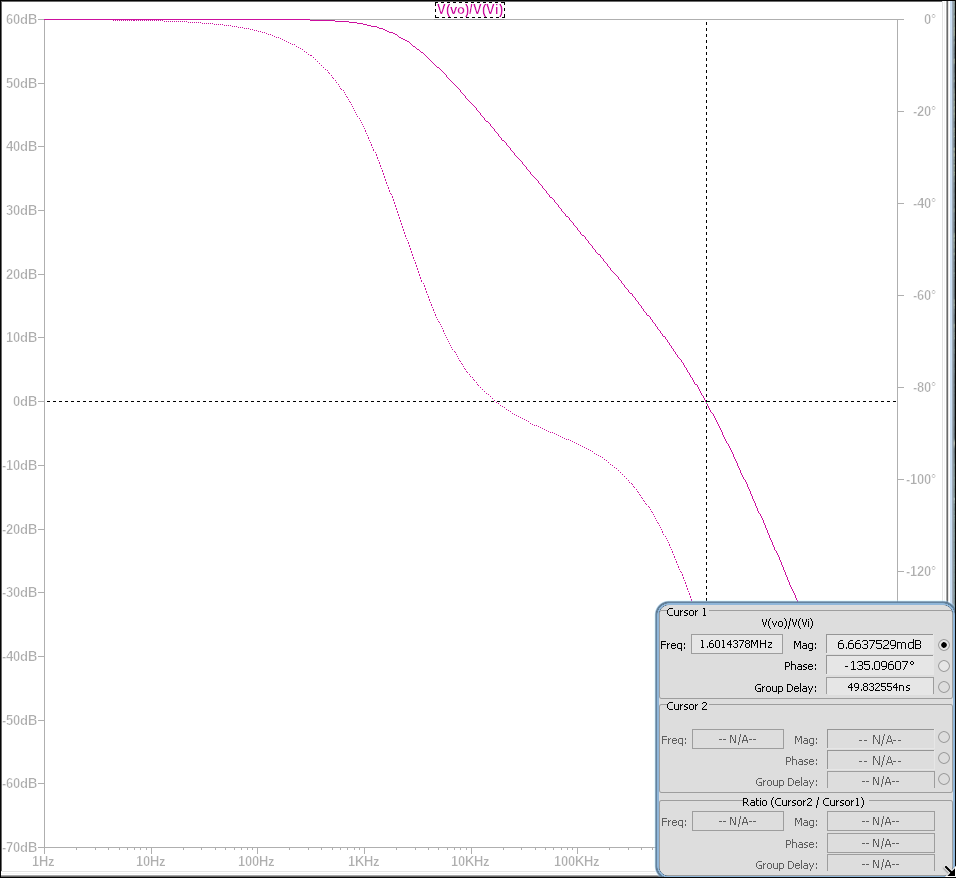
\includegraphics[width=0.9\textwidth]{Imagenes/PMSim14pSinCircuito.png}
    \caption{Simulación de la compensación con efecto Miller}
    \label{fig:sim2}
\end{figure}

\vspace{2em}

\noindent\textbf{Comentarios sobre la estabilidad:}
\vspace{3em}

Este capacitor permite, sin modificar el diseño del circuito aprovechar la alta ganancia en la etapa para evitar la oscilación, obteniendo el comportamiento deseado.